\chapter{Problématiques}
\section{Cadre d'utilisation de Gatling}
La cible première de Gatling est l'ensemble des applications web modernes. Cela signifie que l'outil doit pouvoir envoyer des requêtes sur le protocole HTTP ou HTTPS et fournir la possibilité de simuler des requêtes AJAX\footnote{AJAX signifie \en{Asynchronous Javascript And XML} : Javascript et XML Asynchrones}. Dans les évolutions suivantes, il est prévu de supporter les applications réalisées avec le framework GWT ou avec Flex. Plus tard encore, il est prévu l'ajout de modules permettant de tester des serveurs de données, des annuaires LDAP, etc.

Afin d'offrir des tests ayant une réelle valeur aux yeux des testeurs, mais aussi de leurs dirigeants, Gatling effectuera des simulations d'utilisateurs réalisant des scénarios établis par le testeur. La difficulté de ce genre de test réside dans la rédaction des scénarios, qui doivent être bien faits pour représenter au mieux la réalité.

Si l'écriture des scénarios est laissée aux testeurs, Gatling tentera de simplifier au maximum cette écriture, afin de permettre au testeur de se concentrer sur le contenu de ses scénarios plutôt que sur la façon dont il devra les écrire. 

\section{Ecriture de scénarios}
L'écriture des scénarios doit donc être fluide, et le plus naturelle possible pour le testeur. Cela passe donc par deux choses : l'interface de l'outil et le vocabulaire utilisé.

\subsection{Interface de l'outil}
L'interface de l'outil doit être la plus simple possible afin de ne pas rendre son utilisation trop complexe. Elle peut être graphique, comme les outils présentés plus haut dans ce rapport, ou alors en ligne de commande. 

Gatling étant amené à être exécuté sur des serveurs, sans interface graphique, il semble logique de privilégier l'interface par ligne de commande. Celle-ci pourrait d'ailleurs rebuter les utilisateurs peu expérimentés de l'outil, cependant, le test de charge est souvent réalisé par des personnes qui connaissent bien l'environnement informatique, soit parce qu'ils développent (ce sont parfois les développeurs eux-mêmes qui font ce travail), ou parce qu'ils administrent des serveurs.

\subsection{Utilisation d'un DSL}
L'utilisation de la ligne de commande seule limite considérablement les possibilités de création d'un scénario. En effet, on ne peut fournir d'outils graphiques comme le font JMeter et LoadUI. Cependant, il existe un moyen efficace d'écrire des scénarios : les \em{DSL}. Un DSL, ou \en{Domain Specific Language}, permet de représenter un problème particulier, ou, dans le cas de Gatling, un scenario, ou une simulation.

L'utilisation de DSL apporte plusieurs avantages :
\begin{itemize}
  \item \em{Langage naturel}. Un DSL bien écrit permet d'écrire de façon quasiment naturelle ce que l'on veut représenter. En effet, si le nom des méthodes est bien choisi, on peut parfois écrire des phrases en anglais qui seront interprétées par l'ordinateur, car ces phrases sont composées de méthodes et de paramètres. Ainsi, il est possible d'utiliser des mots proches du domaine concerné par le DSL. En voici un exemple simple dans le cadre des mathématiques :
  \begin{lstlisting}
  // Creates a point named A with coordinates (2, 6)
  createPoint "A" withAbscissa 2 andOrdinate 6;
  \end{lstlisting}
  \item \em{Utilisation des fonctions de base d'un langage}. Etant donné qu'un DSL est écrit avec un langage de programmation et compilé (ou exécuté en tant que script), on peut naturellement y utiliser toutes les fonctionnalités apportées par le langage si besoin. En effet, supposons que l'on veuille créer un point avec une ordonnée avec une valeur égale à deux fois la valeur de l'abscisse, on pourra écrire :
  \begin{lstlisting}
  int x = 3;
  // Creates a point named A with coordinates (x, 2x)
  createPoint "A" withAbscissa x andOrdinate 2*x;
  \end{lstlisting}
  \item \em{Autocomplétion}. L'utilisation d'un langage de programmation afin d'écrire des DSL permet aussi d'utiliser les fonctionnalités que peut offrir un IDE. En effet, l'IDE pourra aider à l'écriture du code utilisant le DSL en proposant les mots disponibles à l'utilisateur lors de l'écriture du code.
\end{itemize}

L'utilisation d'un DSL permettra donc aux utilisateurs de Gatling de bénéficier d'une façon simple et efficace d'écrire leurs scénarios.

\section{Performances}
\subsection{Modèle actuel}
Dans la section \ref{pb_perfs}, la mise en cause des performances des outils de test actuels a été évoquée. En effet, lorsque ces outils veulent simuler des utilisateurs, ils adoptent comme modèle 1 utilisateur = 1 Thread. Cette approche apparait la plus naturelle, et permet de simuler les temps de pause utilisateur en mettant directement les threads en sommeil.

Cette façon de procéder donne généralement des résultats satisfaisants lorsque le nombre d'utilisateurs n'est pas très élevé et le travail de chaque thread relativement simple. Dès que le nombre d'utilisateurs croît ou que le scénario demande un traitement des réponses important, l'exécution de la simulation devient imprévisible. Les temps de pause peuvent parfois varier du simple au double, et le scénario simulé pert ainsi de sa valeur, car il ne correspond pas à ce que souhaitait le testeur. 

\subsection{Les acteurs}
La programmation concurrente est généralement faite en utilisant des threads. On doit donc faire attention à la synchronisation des méthodes, bien veiller à ce que l'on n'ait pas de situation de compétition entre les threads, et, tout faire pour éviter les dead-locks. Programmer en utilisant des threads peut donc vite devenir complexe.

Pour pallier cette complexité, on peut utiliser un modèle dit \em{modèle d'acteur}. Ce modèle, comme l'indique Wikipedia, \begin{quote}est un modèle mathématique qui définit les acteurs comme les seules entités nécessaires au calcul concurrent. En réponse à un message, un acteur effectue un traitement, crée d'autres acteurs et envoie d'autres messages.\end{quote}

Ainsi, la programmation concurrente à l'aide d'acteurs est basée sur l'envoi de messages et des traitements asynchrones. Un acteur est composé d'une \em{unité de calcul} et d'une \em{messagerie}, comme illustré dans la figure \ref{actor}.

\begin{figure}[h]
\begin{center}
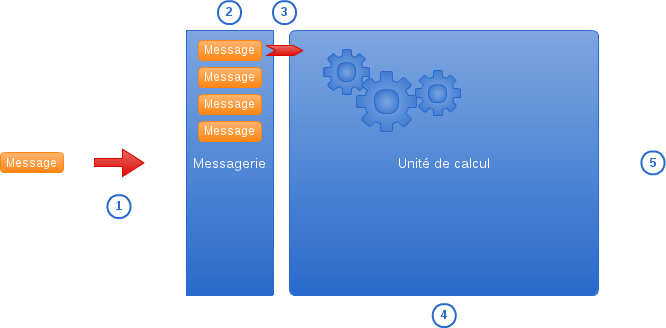
\includegraphics[width=400pt]{img/acteur.png}
\end{center}
\caption{Composition d'un acteur}
\label{actor}
\end{figure}

Le fonctionnement de ce modèle est le suivant :
\begin{enumerate}
  \item Un message est envoyé à l'acteur. Ce message est un ordre donné à l'acteur, il contient, si besoin, les paramètres nécessaires au calcul que l'acteur doit effectuer ;
  \item Le message est stocké dans la messagerie de l'acteur, dans une file d'attente ;
  \item Lorsqu'il y a un message dans la messagerie, l'acteur le traite, il est supprimé de la file d'attente ;
  \item Le traitement de l'ordre contenu dans le message est effectué par l'unité de calcul ;
  \item Enfin, l'acteur peut passer directement au message suivant, ou envoyer des messages à d'autres acteurs avant de passer au message suivant comme illustré par la Figure \ref{actors}.
\end{enumerate}

\begin{figure}[h]
\begin{center}

\includegraphics[width=400pt]{img/acteurs.png}
\end{center}
\caption{Enchainement d'acteurs}
\label{actors}
\end{figure}

\subsection{Le modèle de Gatling}
\subsubsection{Les tests}
Gatling doit donc utiliser le modèle le plus performant afin de garantir les performances qu'il veut offrir. Afin de démontrer que l'approche par le modèle d'acteurs est la plus performante, des tests ont été faits pour comparer JMeter et une preuve de concept utilisant ce modèle. Voici le protocole du test :

\begin{itemize}
  \item Un PC avec Processeur 4 coeurs 2.67GHz, JVM lancée avec 2Go de mémoire alloués (Heap) dédié à l'utilisation de l'outil. L'exécution de la simulation a été faite avec 4Go de RAM au départ pour les deux outils, puis à 5Go, étant donné que JMeter consomme beaucoup de RAM ;
  \item Un serveur web apache tournant sur une autre machine servant une seule page de 100ko ne contenant que du texte ;
  \item Un scénario type : L'utilisateur appelle la page un certain nombre de fois, en effectuant une pause entre chaque appel. Ce nombre de pauses induit une durée de simulation incompréssible de 10mn04s ;
  \item Deux types d'opérations sur la réponse du serveur\footnote{Le fait d'effectuer une opération sur la réponse du serveur permet de tester la robustesse de l'outil face à de telles demandes lorsque leur nombre augmente.} :
  \begin{itemize}
    \item Recherche par \em{expression régulière} ;
    \item Recherche par \em{XPath}.
  \end{itemize}
\end{itemize}

Les résultats de ces tests, consignés dans le tableau \ref{result_tests}, indique que le modèle d'acteurs est bien plus performant que le modèle utilisé par JMeter. En effet, JMeter consomme plus de mémoire vive, et la simulation sur JMeter est parfois bien plus longue qu'avec la preuve de concept. De plus, en surveillant l'activité des coeurs du processeur, on remarque qu'avec la preuve de concept, l'utilisation des coeurs est régulière et oscille autour de 50/60\%, alors que pour JMeter, les coeurs sont très sollicités, avec des pics réguliers à 100\%.

\begin{center}
\begin{table}
\rowcolors{2}{cyan!20!white}{orange!20!white}
\begin{tabular}{c c c c c c l}
\em{Utilisateurs} & \em{RAM} & \em{Opération} & \em{Durée PoC} & \em{Durée JMeter} & \em{Diff.}\\ \hline
2000 & 4Go & RegExp & 10'08'' & 10'21'' & 13''\\
3000 & 4Go & RegExp & 10'11'' & 12'01'' & 1'50''\\
2000 & 4Go & XPath & 10'12'' & 13'08'' & 2'56''\\
2000 & 5Go & XPath & 10'14'' & 10'45'' & 31''\\
3000 & 5Go & XPath & 10'20'' & 18'36'' & 8'16''\\
\end{tabular}
\caption{Résultat des tests modèle d'acteurs vs threads}
\label{result_tests}
\end{table}
\end{center}

L'utilisation du modèle d'acteurs pour le moteur de simulation de Gatling est donc un bon choix et présage un gain de performances non négligeable pour des scénarios complexes qui demandent des opérations gourmandes sur les réponses reçues.

\section{Langage de Gatling}
Il reste une dernière réponse à fournir : en quel langage Gatling doit-il être codé ?

Afin de réaliser Gatling, nous avons besoin d'un langage qui ait :
\begin{itemize}
  \item Une bibliothèque d'acteurs performante et assez mature. En effet, ce modèle, bien que découvert il y a déjà longtemps, n'est pas encore très répandu dans le monde informatique professionnel.
  \item Une syntaxe autorisant la création de DSL \em{simplement}. Il n'existe pas beaucoup de langages qui permettent de s'affranchir des éléments de syntaxe qui rendent le code moins naturel tels que ., \{, \}, (, ), etc.
  \item Une compatibilité avec la JVM. En effet, eBusiness Information travaillant dans les technologies Java/JEE, et la plupart des SI d'entreprise fonctionnant avec Java, il est naturel de proposer un logiciel qui fonctionnera sans avoir à installer des dépendances supplémentaires.
\end{itemize}

Ainsi, nous avons porté notre choix sur le langage \em{Scala}. En effet, ce langage répond aux exigences exprimées ci-dessus et propose même une compatibilité avec toutes les bibliothèques Java ! Cela permet donc de bénéficier d'un langage fonctionnel et objet, tout en ayant accès aux bibliothèques connues de Java. Le listing \ref{exp_scala} montre un exemple de syntaxe Scala abrégée.

\begin{lstlisting}[caption={Exemple de code Scala},label=exp_scala]
object HelloWorld {
  def main(args: Array[String]) {
    println("Hello, world!")
  }
}
\end{lstlisting}

La bibliothèque pour le modèle d'acteurs se nomme \em{Akka}. Ses créateurs ont rejoint l'entreprise TypeSafe qui édite le langage Scala, la bibliothèque sera donc maintenue et bénéficiera de l'expertise des créateurs de Scala. Elle est, de plus, Open Source.